\cleardoublepage
\chapter{Background and Related Work}
\label{cha:background}
The main contributions of this thesis revolve around the SimRa project (see section~\ref{subsec:simra}), which is a crowdsourcing/crowdsensing citizen science application, with the goal of improving cycling comfort and cycling safety.
In this chapter, we go through fundamental topics that are needed to better understand the nature of the SimRa project and thus, the contributions outlined in chapter~\ref{cha:contributions}.
For this, we first outline which factors mainly influence cycling comfort and give an overview of recent studies from that research area in section~\ref{sec:cycling_comfort_background}.
We then continue with cycling safety in section~\ref{sec:cycling_safety_background}, which is related to cycling comfort.
There, we also differentiate between bicycle safety and bicycle traffic safety.
In chapter~\ref{sec:crowdsourcing_crowdsensing_background}, we point out similarities and differences between crowdsourcing and crowdsensing, so that we can later, in section~\ref{subsec:simra}, better categorize the SimRa project between them.
Lastly, to complete this chapter, we take a brief look into the field of citizen science, namely what makes a project a citizen science project, which benefits and challenges it brings and how the related work makes use of it in chapter~\ref{sec:citizen_science_background}. 

\section{Cycling Comfort}
\label{sec:cycling_comfort_background}

\section{Cycling Safety}
\label{sec:cycling_safety_background}

\section{Crowdsourcing and Crowdsensing}
\label{sec:crowdsourcing_crowdsensing_background}
Crowdsourcing and crowdsensing have emerged as successful approaches to solve tasks in a fast and cost-efficient way and gather big amounts of data in a short time respectively.

\subsection*{Crowdsourcing}
``Crowdsourcing'' is a combination of the words \textit{crowd} and \textit{outsourcing}~\cite{howe2006rise}.
\textit{Crowd} refers to an often larger group of individuals, to which a task is transferred to, whereas outsourcing refers to a practice where an entity does not fulfill a task in-house on it's own, but hires people from outside to solve a task for them.
Crowdsourcing comes in many shapes and forms and can be found in many different areas, from transportation, to financing, from social media to natural crisis relief, etc.
A very common form of crowdsourcing is the so called mobile crowdsourcing.
The difference is that in mobile crowdsourcing the the people fulfilling the task usually do not have to be stationary, but rather mobile, because the task at hand demands movement or being in a specific location to be fulfilled~\cite{phuttharak2018review}.
In the latter case, a smartphone or a hardware device fitted with sensors has to be used by the participants to fulfill the task.
For the remainder of this work, we will use the terms crowdsourcing and mobile crowdsourcing interchangeably.

Figure~\ref{fig:crowdsourcing} shows the key elements of crowdsourcing.
In the top layer, the application user (e.g., a ride-hailing app user) requests a task (e.g., a ride from location A to location B).
The data processing platform layer receives this task and determines to whom (e.g., which taxi drivers) to allocate it to.
Then, the crowd (e.g., the taxi driver, that accepts the task) carries it out.
After that, the data processing layer receives the result (e.g., the arrival of the customer at the destination), processes and aggregates it and the sends the end result to the application (e.g., invoice).
In crowdsourcing, it is also possible and sometimes even necessary that the crowd has to collaborate to fulfill the task (e.g., multiple taxi drivers transporting a large group of customers from A to B).

\begin{figure}[htbp]
  \centering
  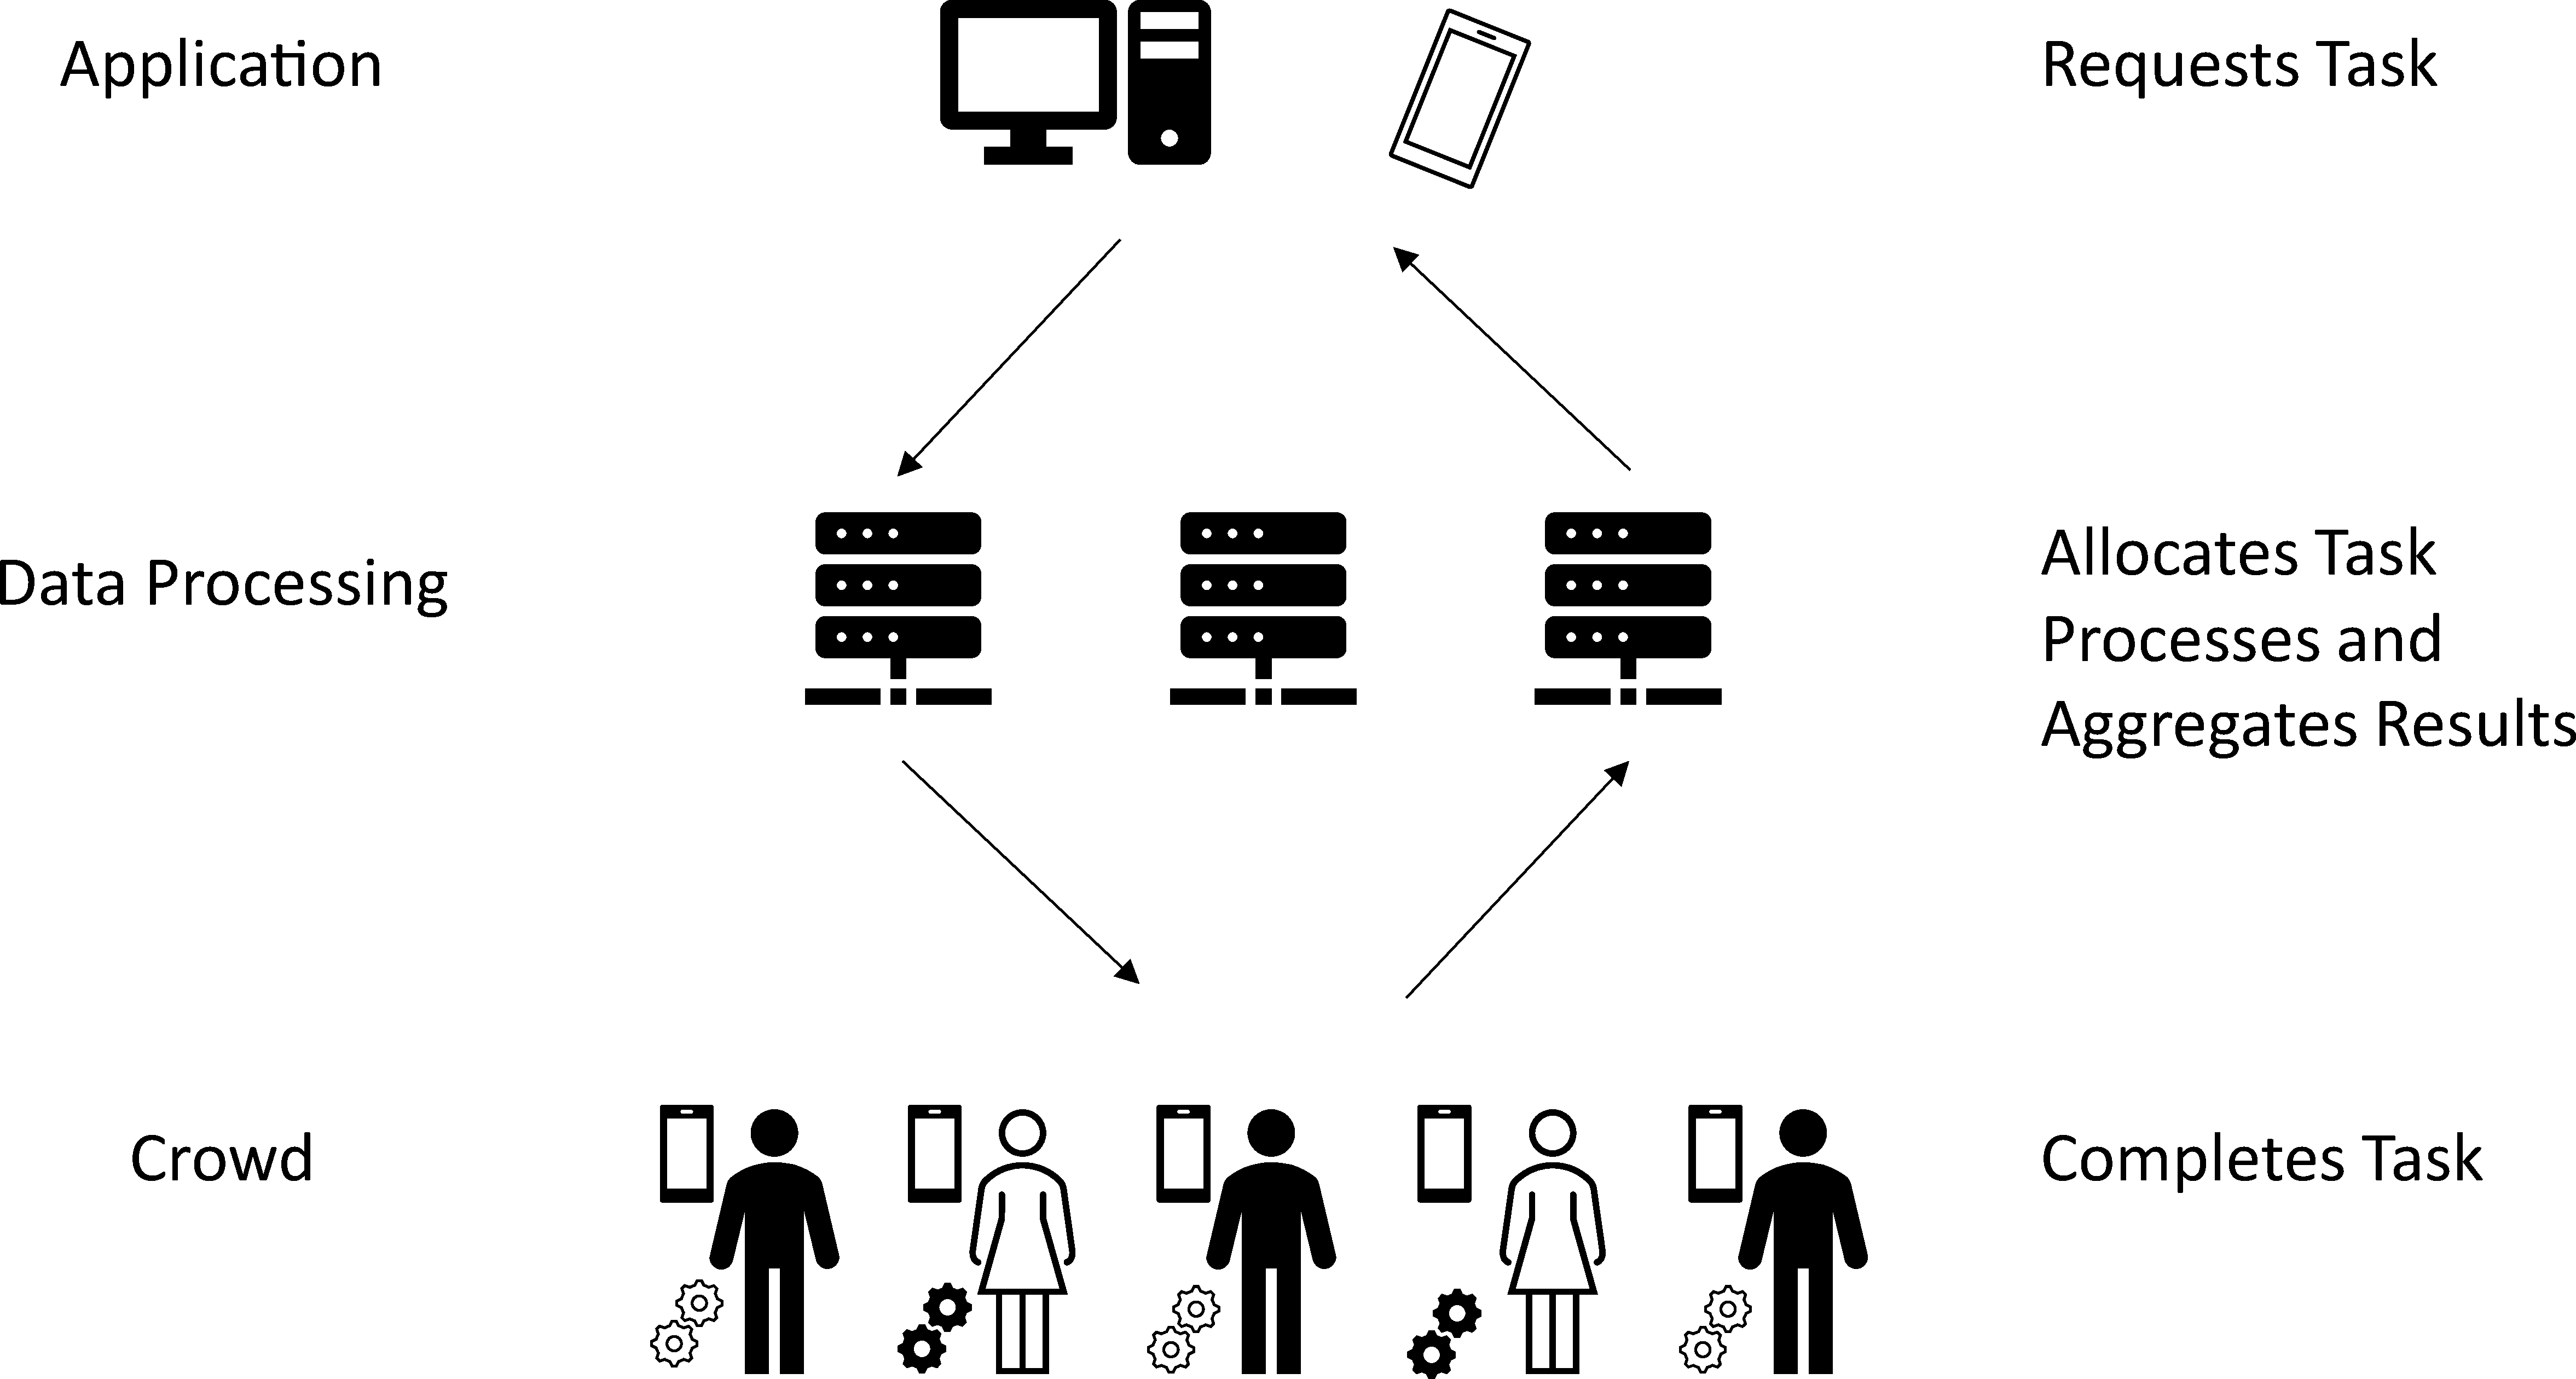
\includegraphics[width=0.8\textwidth]{fig/crowdsourcing.pdf}
  \caption{Crowdsourcing architecture consist of three layers: Application, Data Processing and Crowd}
\end{figure}
\label{fig:crowdsourcing}

There are different aspects that characterize a crowdsourcing application: \textit{degree of human involvement}, \textit{location relevance}, \textit{knowledge requirement}, \textit{participation incentive} and \textit{data flow}~\cite{ray2023survey,kong2019mobile}.

There are two types of \textit{degree of human involvement}: Opportunistic and Participatory.
The former describes that the participant does not actively operate the smartphone or device, while in the latter, he/she has to give further input on the smartphone or device.
The \textit{degree of human involvement} is a continuum, where each crowdsourcing application can have different levels of human involvement.

\textit{Location relevance} refers to the importance of solving a task in a particular location.
With mobile crowdsourcing, a certain degree of \textit{location relevance} is naturally given, but there can still be different levels of \textit{location relevance}.
For instance, the task may need to be completely done at a specific locations, or only parts of it, such as taking a photo of a location but then editing the photo anywhere.
Similar to the \textit{degree of human involvement}, here we also have a continuum, being between high location relevance and no location relevance at all.

\textit{Knowledge requirement} refers to the level of knowledge that the participant needs to fulfill a given task.
Some tasks may be very simple, where detailed knowledge is unnecessary, while other tasks may need some experts of a specific topic or an extensive training to be able to solve the task.
A high \textit{knowledge requirement} may make it necessary to distinctively allocate the task to such participants, where the \textit{knowledge requirements} are met.

The \textit{participation incentive} can vary from project to project and also from participant to participant.
There are basically two types of incentives: intrinsic and extrinsic.
A participant with an intrinsic incentive engages with a crowdsourcing project, because he/she can identify with the problem the project wants to solve or simply likes to to perform the task.
There can also be extrinsic motivations such as getting paid in cash or with coupons, or gaining social credits for it.
It is very much possible, that participants have both intrinsic \textit{and} extrinsic incentives to contribute a project.

The \textit{data flow} is a technical aspect of the crowdsourcing project.
Here, there are three distinctions: centralized, decentralized and hybrid.
When the data flows from the crowd directly to the processing platform, the project has a centralized data flow.
Contrary to that, when the data flow is decentralized, it means that some participants' devices collect results of the solved tasks within the crowd and then send it in aggregated form to the processing platform.
This may be beneficiary to decrease the load on the processing platform.
A hybrid form is also possible, where the crowd or the crowd's devices process the data themselves and send it directly to the application, which makes the processing layer superfluous. 

\subsection*{Crowdsensing}
As in ``crowdsourcing'' the crowd in ``crowdsensing'' refers to a group of people, who voluntarily take over a task.
However, in crowd\textit{sensing}, the task at hand is mainly gathering data for the client, or in other words, \textit{sensing}.
Due to the similar nature of both, the architecture of crowdsensing projects is usually very similar to that of crowdsourcing projects (see figure~\ref{fig:crowdsourcing}).
The main difference from a software architectural view is that the participants usually do not collaborate and thus there is no need for the smartphones and devices in the crowd to communicate with each other.

The characterization is also very similar, although there is usually no \textit{knowledge requirement} aspect in \textit{crowdsensing} projects.
However, there are two additional aspects, that can be used to characterize: \textit{application type} and \textit{data collection}.

There are mainly three \textit{application types}: environmental applications, infrastructure applications and social applications~\cite{ganti2011mobile}.

In \textit{environmental applications}, the goal of the crowdsensing project is to gather data about the \textit{natural} environment.
Examples of \textit{environmental applications} are projects to measure air pollution~\cite{hasenfratz2012participatory,sivaraman2013hazewatch,liu2018third} or monitor water quality~\cite{minkman2015citizen,rapousis2016performance,shang2023crowdwatersens}.

\textit{infrastructure applications} are about gaining insights into the state of public infrastructure.
Common use cases are gathering data about car parking spaces~\cite{villanueva2015crowdsensing,coric2013crowdsensing,rinne2014mobile} or traffic flow~\cite{wang2018city,li2019privacy,mei2020towards}.

As the name suggests, \textit{social applications} gather information about persons and social interactions.
With the help of social media networks, it is possible to extract information from the communications of the crowd~\cite{grasso2017public,cecilia2020mobile,phan2019drinks}, while there is also a focus on mass events~\cite{rahman2017location,cardone2014crowdsensing,jarvis2013ubicomp}.

The \textit{data collection} can come in two forms: \textit{mobile sensing} and \textit{user generated}~\cite{pietschmann2008croco}.

In \textit{mobile sensing} the smartphone or sensing device collects the data automatically.
The participant may need to start an app or turn on a device to start a recording of the sensor data.
When the smartphone or device that collects the data sends the collected data to the data processing platform autonomously, the data collection is \textit{push based}, otherwise, if the data processing platform requests the collected data from an endpoint it is called \textit{pull based}. 

\section{Citizen Science}
\label{sec:citizen_science_background}
Although the term Citizen Science was coined by Irwin~\cite{irwin1995citizen} and Bonney~\cite{bonney1996citizen} in the mid-90s, the concept is much older.
For example, the National Audubon Society's project called ``Christmas Bird Count'', where everyone is invited to participate to count birds and report their findings.
It runs since the year 1900 and can be considered as the first Citizen Science project~\cite{silvertown2009new}.
This can be considered as Citizen Science because it is a scientific endeavor, where anyone can participate, which is the broadest way to describe Citizen Science.
However, since the emergence of the term ``Citizen Science'' different definitions have been proposed by different scientific, social and political parties~\cite{heigl2019toward,ecsa2015ten,us2016crowdsourcing} and there is an active discussion of what can be considered as a Citizen Science Project and what cannot~\cite{haklay2021citizen}. 

Haklay et al. compiled a list of 32 definitions for Citizen Science from different reference sources, citizen science associations, global multinational organizations and different governmental bodies~\cite{haklay2021citizen}.
One of their key findings that although most definitions have descriptive, instrumental and normative elements, the weighting can differ according to the goals of the proposing party of the definition.
\textit{National Geographic} has for example a more descriptive definition:
\begin{quote}
\textit{Citizen science is the practice of public participation and collaboration in scientific research to increase scientific knowledge. Through citizen science, people share and contribute to data monitoring and collection programs.}
\end{quote}
After a broad description of what Citizen Science is, it underlines ``data monitoring and collection'' which is not surprising for a environmental-focused organization.

The \textit{US National Institutes of Health} chooses a more instrumentalist approach when defining Citizen Science:
\begin{quote}
\textit{Citizen science efforts are driven by community concerns. These community-led projects may involve a partnership with an academic or research institution, where both parties work together to collect and share data. The goal is to address a community concern through collaborative research and to translate the research findings into public health action that benefits the community.}
\end{quote}
The last sentence of their definition clearly puts a focus on public health, which is not understandable from their point of view.
There are also definitions who try to be normative, such as the definition from UNESCO:
\begin{quote}
\textit{[Citizen Science:] The participation of a range of non-scientific stakeholders in the scientific process. At its most inclusive and most innovative, citizen science involves citizen volunteers as partners in the entire scientific process, including determining research themes, questions, methodologies, and means of disseminating results.}
\end{quote}
It is remarkable that this definition mentions inclusiveness and voluntarism.

Eitzel et al.~\cite{eitzel2017citizen} also analyze different definitions of Citizen Science and identify three categories: Citizen Science as a \textit{tool}, a \textit{movement} or a \textit{social capacity}.
Accordingly, Citizen Science can be seen as a\textit{tool} to help answering a research question, e.g. by gathering data.
On the other hand, Citizen Science can also be seen as a \textit{movement} to democratize science and thus increase the trust of the society in science.
Finally, Citizen Science can be seen as a \textit{social capacity} to increase evidence-based decision making.

The European Citizen Science Association (ECSA)~\footnote{https://www.ecsa.ngo/} contributes the ten principles of citizen science~\cite{ecsa2015ten}:

\begin{enumerate}
\item \textit{Citizen science projects actively involve citizens in scientific endeavour that generates new
knowledge or understanding. Citizens may act as contributors, collaborators, or as project
leader and have a meaningful role in the project.}
\item \textit{Citizen science projects have a genuine science outcome.} For example, answering a research
question or informing conservation action, management decisions or environmental policy.
\item \textit{Both the professional scientists and the citizen scientists benefit from taking part.} Benefits
may include the publication of research outputs, learning opportunities, personal enjoyment,
social benefits, satisfaction through contributing to scientific evidence e.g. to address local,
national and international issues, and through that, the potential to influence policy.
\item \textit{Citizen scientists may, if they wish, participate in multiple stages of the scientific process.} This may include developing the research question, designing the method, gathering and
analysing data, and communicating the results.
\item \textit{Citizen scientists receive feedback from the project.} For example, how their data are being used
and what the research, policy or societal outcomes are.
\item \textit{Citizen science is considered a research approach like any other, with limitations and biases
that should be considered and controlled for.} However unlike traditional research approaches,
citizen science provides opportunity for greater public engagement and democratisation of
science.
\item \textit{Citizen science project data and meta-data are made publicly available and where possible,
results are published in an open access format.} Data sharing may occur during or after the
project, unless there are security or privacy concerns that prevent this.
\item \textit{Citizen scientists are acknowledged in project results and publications.}
\item \textit{Citizen science programmes are evaluated for their scientific output, data quality, participant
experience and wider societal or policy impact.}
\item \textit{The leaders of citizen science projects take into consideration legal and ethical issues
surrounding copyright, intellectual property, data sharing agreements, confidentiality,
attribution, and the environmental impact of any activities.}
\end{enumerate}

The plethora of different definitions, guidelines and principles show that Citizen Science is a broad term that can be interpreted according to the circumstances.
This, however, is also a benefit, since it allows different projects to label themselves as Citizen Science and get funding from different organizations and national institutions.




%
%% There are MANY definitions. https://doi.org/10.1073/pnas.1909278116 and https://doi.org/10.5281/zenodo.3552753 compiled lists of them.
%% https://doi.org/10.5334/cstp.230 analyzed definitions.
%% Definitions have descriptive, instrumental, and normative aspects (https://link.springer.com/chapter/10.1007/978-3-030-58278-4_2#Sec2)
%% epistemology, methodology, and social practice and possible impacts on the given context of application.
%% aspects of citizen science: open data, open participation, voluntarity, open source, hierarchy
%% 5 types of citizen science projects: Action, Conservation, Investigation, Virtual, Education
%% 
%% From Citizen science: crowdsourcing for research Catherine Lichten
%% Citizen science projects also present an opportunity to involve non-researchers in the scientific process and for researchers to interact with the wider community. Involving the public in research can help to improve scientific understanding and literacy, and enhance public trust in science (Garbarino J., & C.E. Mason. 2016. ‘The Power of Engaging Citizen Scientists for Scientific Progress.’ Journal of Microbiology and Biology Education 17 (1): 7–12.)
%%
%% Three views on 'Citizen Science' (from Eitzel https://doi.org/10.5334/cstp.96):
%% 1) Instrumental, as a tool, method, or form of research collaboration  (e.g., Bonney et al. 2009b; Wiggins and Crowston 2011; Follett and Streznov 2015)
%% 2) a movement that democratizes the scientific research process (Irwin 1995)
%% 3) Social Capacity / knowledge-producing capacity of society and a path to evidence-based decision-making (Nielsen 2011)
%%
%% It is important to note that despite their reliance on micro-tasking and light engagement, there is evidence (Eveleigh et al. 2014) that some participants use the opportunity to develop deeper interest and engagement in science.
%%
%%
%%
%%
%%
%